% Options for packages loaded elsewhere
\PassOptionsToPackage{unicode}{hyperref}
\PassOptionsToPackage{hyphens}{url}
%
\documentclass[
  12pt,
]{article}
\usepackage{amsmath,amssymb}
\usepackage{lmodern}
\usepackage{ifxetex,ifluatex}
\ifnum 0\ifxetex 1\fi\ifluatex 1\fi=0 % if pdftex
  \usepackage[T1]{fontenc}
  \usepackage[utf8]{inputenc}
  \usepackage{textcomp} % provide euro and other symbols
\else % if luatex or xetex
  \usepackage{unicode-math}
  \defaultfontfeatures{Scale=MatchLowercase}
  \defaultfontfeatures[\rmfamily]{Ligatures=TeX,Scale=1}
\fi
% Use upquote if available, for straight quotes in verbatim environments
\IfFileExists{upquote.sty}{\usepackage{upquote}}{}
\IfFileExists{microtype.sty}{% use microtype if available
  \usepackage[]{microtype}
  \UseMicrotypeSet[protrusion]{basicmath} % disable protrusion for tt fonts
}{}
\makeatletter
\@ifundefined{KOMAClassName}{% if non-KOMA class
  \IfFileExists{parskip.sty}{%
    \usepackage{parskip}
  }{% else
    \setlength{\parindent}{0pt}
    \setlength{\parskip}{6pt plus 2pt minus 1pt}}
}{% if KOMA class
  \KOMAoptions{parskip=half}}
\makeatother
\usepackage{xcolor}
\IfFileExists{xurl.sty}{\usepackage{xurl}}{} % add URL line breaks if available
\IfFileExists{bookmark.sty}{\usepackage{bookmark}}{\usepackage{hyperref}}
\hypersetup{
  hidelinks,
  pdfcreator={LaTeX via pandoc}}
\urlstyle{same} % disable monospaced font for URLs
\usepackage[margin=1in]{geometry}
\usepackage{graphicx}
\makeatletter
\def\maxwidth{\ifdim\Gin@nat@width>\linewidth\linewidth\else\Gin@nat@width\fi}
\def\maxheight{\ifdim\Gin@nat@height>\textheight\textheight\else\Gin@nat@height\fi}
\makeatother
% Scale images if necessary, so that they will not overflow the page
% margins by default, and it is still possible to overwrite the defaults
% using explicit options in \includegraphics[width, height, ...]{}
\setkeys{Gin}{width=\maxwidth,height=\maxheight,keepaspectratio}
% Set default figure placement to htbp
\makeatletter
\def\fps@figure{htbp}
\makeatother
\setlength{\emergencystretch}{3em} % prevent overfull lines
\providecommand{\tightlist}{%
  \setlength{\itemsep}{0pt}\setlength{\parskip}{0pt}}
\setcounter{secnumdepth}{-\maxdimen} % remove section numbering
\usepackage{setspace}/spacing{2}
\usepackage{float}
\usepackage{sectsty}
\usepackage{fancyhdr}
\usepackage{lastpage}
\usepackage[margin=2in]{geometry}
\usepackage{indent first}
\ifluatex
  \usepackage{selnolig}  % disable illegal ligatures
\fi

\author{}
\date{\vspace{-2.5em}}

\begin{document}

\textbackslash begin\{document\} \allsectionsfont{\centering}
\subsectionfont{\raggedright} \subsubsectionfont{\raggedright}

\pagenumbering{gobble}

\begin{centering}
\vspace{24pt}
Final Paper
Claire Guidinger & Yijun Cheng
EDLD 651
\end{centering}

\newpage

\begin{centering}
**Abstract**
\end{centering}

\newpage
\spacing{2}

\hypertarget{introduction}{%
\section{\texorpdfstring{\textbf{Introduction}}{Introduction}}\label{introduction}}

Historically, men have been understudied and underrepresented in
disordered eating research (Braun et al., 1999; Lavender et al., 2017).
Yet, increasing and compelling data indicate that young men between the
ages of 18-30, in particular, report high rates of disordered eating
symptoms (Braun et al., 1999; Strother et al., 2012). Excessive exercise
and muscularity-enhancing behaviors may be especially applicable to
young men, given the current sociocultural pressures for young men to
embody the mesomorphic body ideal (e.g., a lean and muscular physique)
(Lavender et al., 2017). Indeed, many men report being dissatisfied with
their bodies and a desire to reduce their fat mass and increase their
muscle mass (Pope, Phillips, \& Olivardia, 2000; Baghurst, Hollander,
Nardella, \& Haff, 2006). Excessive exercise aimed at enhancing
muscularity may function to reduce body dissatisfaction while also
simultaneously working towards achieving the mesomorphic body ideal.
Although excessive exercise and muscularity-enhancing behaviors are
rampant in young men (Spann \& Pritchard, 2008), little is known about
sociocultural risk factors that precipitate and maintain these
behaviors. Extant data suggest that Asian/Asian American men report the
most severe disordered eating symptoms, such as muscularity-enhancing
behaviors, across racial/ethnic groups (Kelly et al., 2015; Strother et
al., 2012). Indeed, Asian/Asian American men often rate their bodies as
smaller than their ideal physique (Barnett et al., 2002). Potential
romantic partners also rate Asian/Asian American men as less masculine
and more feminine than their non-Asian counterparts (Wilkins et al.,
2011). These harmful stereotypes may render Asian/Asian American men
especially susceptible to engaging in muscularity-enhancing behaviors in
an effort to achieve the mesomorphic body ideal. Evidently, harmful
stereotypes have a profound effect on Asian/Asian American men's body
image and associated disordered eating behaviors. Racial discrimination,
in the forms of both overt racism and microaggressions, may be
particularly relevant to Asian/Asian American men's behavioral drive for
muscularity (Nadal et al., 2014). Preliminary data suggest that overt
racism (e.g., ``Asian Americans were historically targets of racism'')
and microaggressions (e.g., ``a student you do not know asks you for
help in math'') are positively associated with disinhibited eating in
young, Asian/Asian American men (e.g., binge eating and loss of control
eating) (Kelly et al., 2018). However, no studies to date have
identified if experiences with overt racism and microaggressions are
linked to muscularity enhancing behaviors, specifically (e.g., body
building, metabolic steroid use, excessive weightlifting) in young
Asian/Asian American men. \#\# \textbf{Study Aims and Hypotheses} This
study seeks to examine the link between experiences with racial
discrimination, both in the forms of overt racism and microaggressions,
in young Asian/Asian American men. It is hypothesized that experiences
with both overt racism and microaggressions will be significantly and
positively associated with the behavioral drive for muscularity (e.g.,
body building, supplement consumption, metabolic steroid use, excessive
weightlifting, etc.). The study hypotheses are as follows: Hypothesis 1:
Experiences with overt racism will be significantly and positively
associated with the behavioral drive for muscularity in young,
Asian/Asian American men. Hypothesis 2: Experiences with
microaggressions will be significantly and positively associated with
the behavioral drive for muscularity in young, Asian/Asian American men.

\begin{centering}
# **Methods**
\end{centering}

This study was approved by the University of Oregon Institutional Review
Board (IRB). Data were collected between January-February 2017.
Participants were recruited through Qualtrics Panels, which utilize
social media outlets to recruit a diverse sample of survey respondents.
Eligibility criteria included being 18-to-30-years-old; self-identifying
as male and Asian/Asian American; and English fluency. Participants were
asked to complete an online survey. All study responses were anonymous
and considered invalid if less than 80\% of questions were answered
(Dong \& Peng, 2013), the survey was completed in \textless{} 2 minutes
(n = 9), or if participants failed to answer ``yes'' to an embedded
validity item (n = 52). \#\# \textbf{Measures} \emph{Demographics.}
Participants self-reported their age; height (ft, in) and weight (lbs.),
from which body mass index (BMI) in kg/m2 was calculated; ethnicity;
generation status; geographic region; highest education; employment
status; income; geographic region; and presence of a psychiatric
diagnosis. \emph{Experiences with racism.} Participants completed the
13-item Asian American Racism-Related Stress Inventory (Miller et al.,
2012). Items were rated on a 5-point scale from 1 (This has never
happened to me or someone I know) to 5 (This event happened, and I was
extremely upset). Two subscale composite scores were created to measure
experiences with overt racism (e.g., ``You see a TV commercial in which
an Asian character speaks bad English and acts subservient to non-Asian
characters'') and microaggressions (e.g., ``Someone asks you if you can
teach him or her karate''). The Asian American Racism-Related Stress
Inventory (Miller et al., 2012) has been found to have strong
psychometric properties (α = 0.81-0.95). \emph{Behavioral Drive for
Muscularity.} The 15-item Drive for Muscularity Scale (DMS; McCreary \&
Sasse, 2000) will be used to assess the behavioral drive for
muscularity. The DMS measures drive for muscularity across both
cognitive and behavioral dimensions; the construct of interest in the
present study is the behavioral dimension (e.g., ``I lift weights to
build up muscle''). Participants rated the frequency to which they
engage in behaviors with the intention to increase muscularity on a
6-point Likert scale from 1 (never) to 6 (always). A mean score of the
behavioral items was calculated, with higher scores indicating a greater
behavioral drive for muscularity. The DMS has demonstrated good internal
consistency among ethnically diverse adult men (e.g., Swami, 2016).

\begin{centering}
# **Results**
\end{centering}

RStudio Statistical Software was used for all analyses. To ensure data
met model assumptions, data were first screened using the
``Performance'' and ``ggResidpanel'' packages to assess indices of model
quality, goodness of fit, and data missingness. Data fulfilled all model
assumptions and missing data were minimal (\textless2\%), and thus
listwise deletion was employed (Buhi et al., 2008). All analyses
adjusted for BMI, education, income, and presence of psychiatric
diagnosis given a robust body of prior literature identifying
significant, positive associations with disordered eating symptoms
(McLean et al., 2014; Striegel, Bedrosian, Wang, \& Schwartz, 2011). A
linear regression was conducted to examine the link between experiences
with overt racism and the behavioral drive for muscularity. Experiences
with overt racism were significantly and positively associated with the
behavioral drive for muscularity in Asian/Asian American men, F(5, 250)
= 4.06, p \textless{} .01, R2 = 0.08. Experiences with microaggressions
were also significantly and positively associated with the behavioral
drive for muscularity in Asian/Asian American men, F(5, 250) = 6.48, p
\textless{} .001, R2 = 0.12. Findings indicate that as Asian/Asian
American men report greater incidences of both overt racism and
microaggressions, they engage in significantly more
muscularity-enhancing behaviors (e.g., excessive weightlifting, anabolic
steroid use, supplement consumption, etc.).

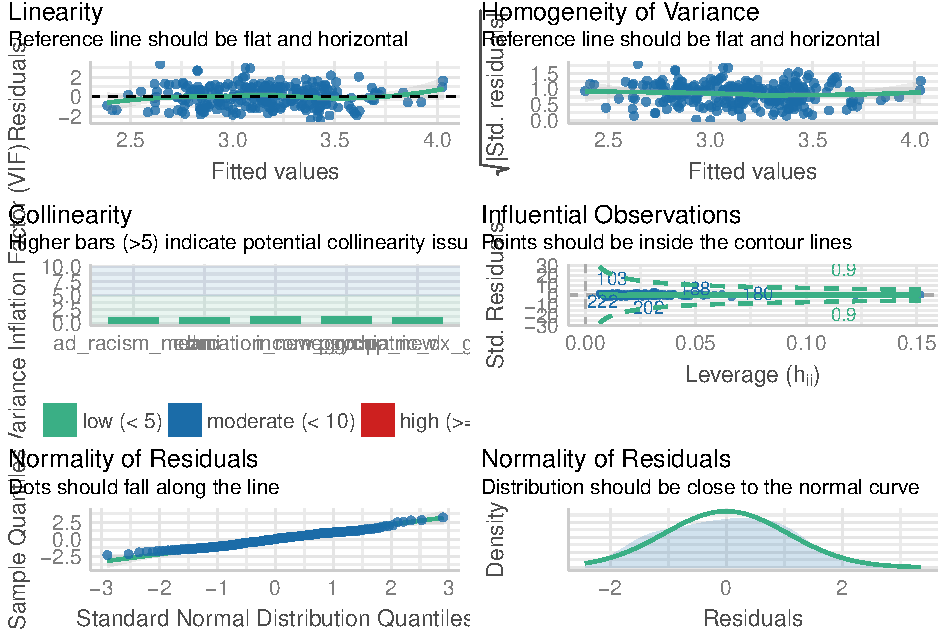
\includegraphics{final_project_files/figure-latex/model_assumptions-1.pdf}

\begin{verbatim}
## 
## Call:
## lm(formula = dms_mean ~ income_group_new + education_new_group + 
##     bmi + psychiatric_dx_group + ad_racism_mean, data = asian_men)
## 
## Residuals:
##     Min      1Q  Median      3Q     Max 
## -2.4296 -0.8159  0.0014  0.7719  3.3548 
## 
## Coefficients:
##                       Estimate Std. Error t value Pr(>|t|)    
## (Intercept)           2.205374   0.398803   5.530 8.05e-08 ***
## income_group_new      0.094716   0.056726   1.670 0.096229 .  
## education_new_group  -0.040695   0.090255  -0.451 0.652461    
## bmi                   0.004074   0.012342   0.330 0.741620    
## psychiatric_dx_group -0.220569   0.171103  -1.289 0.198556    
## ad_racism_mean        0.274068   0.075004   3.654 0.000315 ***
## ---
## Signif. codes:  0 '***' 0.001 '**' 0.01 '*' 0.05 '.' 0.1 ' ' 1
## 
## Residual standard error: 1.075 on 250 degrees of freedom
##   (10 observations deleted due to missingness)
## Multiple R-squared:  0.07514,    Adjusted R-squared:  0.05664 
## F-statistic: 4.062 on 5 and 250 DF,  p-value: 0.001458
\end{verbatim}

\begin{verbatim}
## 
## Call:
## lm(formula = dms_mean ~ income_group_new + education_new_group + 
##     bmi + psychiatric_dx_group + ad_microaggr_mean, data = asian_men)
## 
## Residuals:
##     Min      1Q  Median      3Q     Max 
## -2.8897 -0.7339  0.0185  0.7094  3.3881 
## 
## Coefficients:
##                       Estimate Std. Error t value Pr(>|t|)    
## (Intercept)           2.099064   0.385157   5.450 1.21e-07 ***
## income_group_new      0.107461   0.055032   1.953    0.052 .  
## education_new_group  -0.044491   0.088309  -0.504    0.615    
## bmi                   0.002432   0.012083   0.201    0.841    
## psychiatric_dx_group -0.160033   0.166991  -0.958    0.339    
## ad_microaggr_mean     0.383180   0.076431   5.013 1.01e-06 ***
## ---
## Signif. codes:  0 '***' 0.001 '**' 0.01 '*' 0.05 '.' 0.1 ' ' 1
## 
## Residual standard error: 1.051 on 250 degrees of freedom
##   (10 observations deleted due to missingness)
## Multiple R-squared:  0.1147, Adjusted R-squared:  0.09704 
## F-statistic: 6.481 on 5 and 250 DF,  p-value: 1.098e-05
\end{verbatim}

\begin{centering}
# **Discussion**
\end{centering}

This was the first known study to examine the link between Asian/Asian
American men's experiences with race-related discrimination, both in the
forms of overt racism and microaggressions, and the behavioral drive for
muscularity. As hypothesized, both experiences with overt racism (e.g.,
``You see a TV commercial in which an Asian character speaks bad English
and acts subservient to non-Asian characters'') and microaggressions
(e.g., ``Someone asks you if you can teach him or her karate'') were
significantly and positively associated with the behavioral drive for
muscularity (e.g., engaging in behaviors aimed at increasing muscle
mass). The current study sheds further light on the harmful effects of
racism on Asian/Asian American's mental health, including body image and
disordered eating behaviors. This is particularly pervasive given the
increasingly muscular, mesomorphic male body ideal perpetuated
throughout Western media (Edwards et al., 2016). Extant data suggest
that Asian/Asian American men are often stereotyped to be smaller, more
feminine, less masculine, and less sexually attractive than their
non-Asian peers (Wilkins et al., 2011). As such, it is theorized that
when Asian/Asian American men experience race-related discrimination
(e.g., overt racism and/or microaggressions), their Asian identity
becomes particularly salient, therefore perpetuating internalized
feelings of perceived inadequacy with regards to embodying the
mesomorphic, Western male body ideal. This, in turn, may result in
Asian/Asian American men going to extreme lengths to achieve the ideal
body physique, including excessive and compulsive muscularity-enhancing
behaviors. It is important to consider limitations to the current study,
including the cross-sectional study design. The findings are
correlational, rather than causal, and experimental and prospective data
are needed to determine if experiences with racism prompt
muscularity-enhancing behaviors. While the current study includes a
large, nationally represented sample of Asian/Asian American men, we
were underpowered to examine whether the link between experiences with
race-related discrimination and muscularity-enhancing behaviors vary by
Asian ethnic identity (e.g., Chinese, Japanese, Korean, Asian Indian,
Filipino, and other Asian subgroups). Future research should seek to
clarify whether there are intra- and inter-ethnic variations in these
associations. Although prospective and mechanistic studies are needed,
these findings indicate that experiences with race-related
discrimination negatively impact Asian/Asian American men's body image,
thus prompting engagement in potentially harmful and compulsive
muscularity-enhancing behaviors. The current study adds to a small, but
growing body of research implicating experiences with race-related
discrimination as a significant contributor to health disparities among
racial/ethnic minority men living in the United States. These data may
help to inform clinical programming and preventative interventions aimed
at addressing the harmful effects of race-related discrimination on
men's body image and disordered eating behaviors. The current study may
also help to inform the development and implementation of interventions
aimed at helping Asian/Asian American men adopt healthy coping
strategies in response to discriminatory experiences. Overall, this
study sheds light on the numerous, adverse effects of race-related
discrimination on minority mental health.

```

\end{document}
